% ACL-ready figure for Smokemirror Pipeline
% Copy this into your paper's figure environment

\usepackage{tikz}
\usetikzlibrary{shapes.geometric, arrows.meta, positioning, fit, backgrounds, calc}

% ============================================================
% Figure 1: Compact Pipeline (2x2 Grid Layout) - RECOMMENDED
% ============================================================
\begin{figure*}[t]
\centering
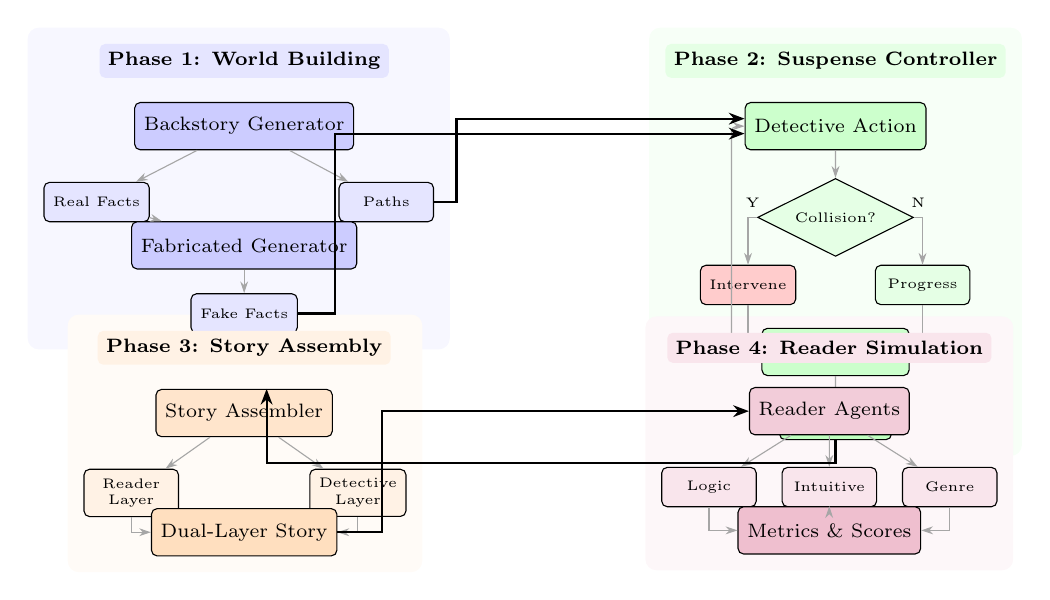
\begin{tikzpicture}[
    node distance=0.3cm and 0.5cm,
    mainbox/.style={rectangle, draw, rounded corners=2pt, minimum width=1.6cm, minimum height=0.6cm, align=center, font=\scriptsize},
    smallbox/.style={rectangle, draw, rounded corners=2pt, minimum width=1.2cm, minimum height=0.5cm, align=center, font=\tiny},
    phaselabel/.style={font=\scriptsize\bfseries},
    decision/.style={diamond, draw, aspect=2, minimum width=0.8cm, font=\tiny},
    arrow/.style={-{Stealth[length=1.5mm, width=1mm]}, draw=gray!70},
    phasearrow/.style={-{Stealth[length=2mm, width=1.5mm]}, thick, draw=black},
    scale=0.95
]

% ============ ROW 1 ============

% PHASE 1: World Building (Top Left)
\node[phaselabel, fill=blue!10, rounded corners=2pt, inner sep=3pt] (p1label) {Phase 1: World Building};
\node[mainbox, fill=blue!20, below=0.3cm of p1label] (backstory) {Backstory Generator};
\node[smallbox, fill=blue!10, below left=0.4cm and -0.2cm of backstory] (realfacts) {Real Facts};
\node[smallbox, fill=blue!10, below right=0.4cm and -0.2cm of backstory] (paths) {Paths};
\node[mainbox, fill=blue!20, below=0.9cm of backstory] (fabgen) {Fabricated Generator};
\node[smallbox, fill=blue!10, below=0.3cm of fabgen] (fabfacts) {Fake Facts};

\draw[arrow] (backstory) -- (realfacts);
\draw[arrow] (backstory) -- (paths);
\draw[arrow] (realfacts) -- (fabgen);
\draw[arrow] (fabgen) -- (fabfacts);

% PHASE 2: Suspense Controller (Top Right)
\node[phaselabel, fill=green!10, rounded corners=2pt, inner sep=3pt, right=3.5cm of p1label] (p2label) {Phase 2: Suspense Controller};
\node[mainbox, fill=green!20, below=0.3cm of p2label] (detective) {Detective Action};
\node[decision, fill=green!10, below=0.35cm of detective] (collision) {Collision?};
\node[smallbox, fill=red!20, below left=0.35cm and 0cm of collision] (intervention) {Intervene};
\node[smallbox, fill=green!10, below right=0.35cm and 0cm of collision] (progress) {Progress};
\node[mainbox, fill=green!20, below=0.9cm of collision] (state) {Update State};
\node[smallbox, fill=green!25, below=0.3cm of state] (plotpoints) {Plot Points};

\draw[arrow] (detective) -- (collision);
\draw[arrow] (collision) -| node[above, font=\tiny, pos=0.25] {Y} (intervention);
\draw[arrow] (collision) -| node[above, font=\tiny, pos=0.25] {N} (progress);
\draw[arrow] (intervention) |- (state);
\draw[arrow] (progress) |- (state);
\draw[arrow] (state) -- (plotpoints);
\draw[arrow, rounded corners=2pt] (state.west) -- ++(-0.4,0) |- (detective.west);

% ============ ROW 2 ============

% PHASE 3: Narrative (Bottom Left)
\node[phaselabel, fill=orange!10, rounded corners=2pt, inner sep=3pt, below=3.2cm of p1label] (p3label) {Phase 3: Story Assembly};
\node[mainbox, fill=orange!20, below=0.3cm of p3label] (assembler) {Story Assembler};
\node[smallbox, fill=orange!10, below left=0.4cm and -0.3cm of assembler] (readerlayer) {Reader\\Layer};
\node[smallbox, fill=orange!10, below right=0.4cm and -0.3cm of assembler] (detlayer) {Detective\\Layer};
\node[mainbox, fill=orange!25, below=0.9cm of assembler] (story) {Dual-Layer Story};

\draw[arrow] (assembler) -- (readerlayer);
\draw[arrow] (assembler) -- (detlayer);
\draw[arrow] (readerlayer) |- (story);
\draw[arrow] (detlayer) |- (story);

% PHASE 4: Evaluation (Bottom Right)
\node[phaselabel, fill=purple!10, rounded corners=2pt, inner sep=3pt, right=3.5cm of p3label] (p4label) {Phase 4: Reader Simulation};
\node[mainbox, fill=purple!20, below=0.3cm of p4label] (readsim) {Reader Agents};
\node[smallbox, fill=purple!10, below left=0.4cm and -0.1cm of readsim] (logic) {Logic};
\node[smallbox, fill=purple!10, below=0.4cm of readsim] (intuitive) {Intuitive};
\node[smallbox, fill=purple!10, below right=0.4cm and -0.1cm of readsim] (genre) {Genre};
\node[mainbox, fill=purple!25, below=0.9cm of readsim] (metrics) {Metrics \& Scores};

\draw[arrow] (readsim) -- (logic);
\draw[arrow] (readsim) -- (intuitive);
\draw[arrow] (readsim) -- (genre);
\draw[arrow] (logic) |- (metrics);
\draw[arrow] (intuitive) -- (metrics);
\draw[arrow] (genre) |- (metrics);

% ============ PHASE CONNECTIONS ============
% Phase 1 -> Phase 2
\draw[phasearrow] (fabfacts.east) -- ++(0.5,0) |- ([yshift=-0.1cm]detective.west);
\draw[phasearrow] (paths.east) -- ++(0.3,0) |- ([yshift=0.1cm]detective.west);

% Phase 2 -> Phase 3
\draw[phasearrow] (plotpoints.south) -- ++(0,-0.3) -| ([xshift=0.3cm]assembler.north);

% Phase 3 -> Phase 4
\draw[phasearrow] (story.east) -- ++(0.6,0) |- (readsim.west);

% ============ Background Boxes ============
\begin{scope}[on background layer]
    \node[fit=(p1label)(backstory)(realfacts)(paths)(fabgen)(fabfacts),
          fill=blue!3, rounded corners=4pt, inner sep=0.2cm] {};
    \node[fit=(p2label)(detective)(collision)(intervention)(progress)(state)(plotpoints),
          fill=green!3, rounded corners=4pt, inner sep=0.2cm] {};
    \node[fit=(p3label)(assembler)(readerlayer)(detlayer)(story),
          fill=orange!3, rounded corners=4pt, inner sep=0.2cm] {};
    \node[fit=(p4label)(readsim)(logic)(intuitive)(genre)(metrics),
          fill=purple!3, rounded corners=4pt, inner sep=0.2cm] {};
\end{scope}

\end{tikzpicture}
\caption{The \textsc{SmokeMirror} pipeline generates dual-layer mystery narratives through four phases: (1) creating ground truth and fabricated cover stories, (2) iteratively generating plot points with collision detection to manage suspense, (3) assembling prose with parallel reader/detective perspectives, and (4) multi-agent evaluation from different reader viewpoints.}
\label{fig:pipeline}
\end{figure*}


% ============================================================
% Figure 1 Alternative: Single Column Vertical Layout
% Use this if you need a single-column figure
% ============================================================
\begin{figure}[t]
\centering
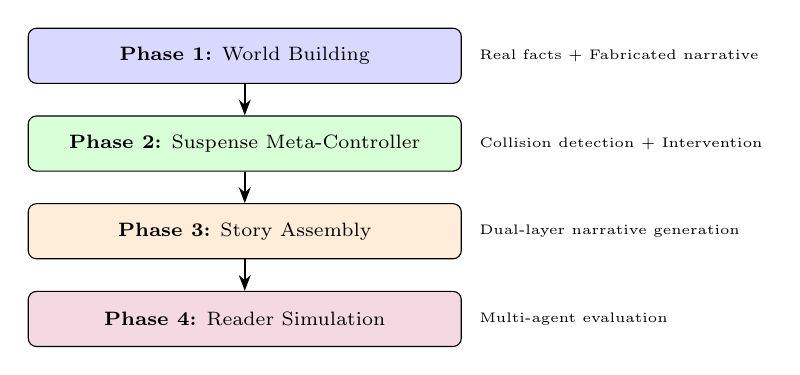
\begin{tikzpicture}[
    node distance=0.25cm,
    phase/.style={rectangle, draw, rounded corners=3pt, minimum width=5.5cm, minimum height=0.7cm, align=center, font=\scriptsize},
    arrow/.style={-{Stealth[length=2mm]}, thick},
    label/.style={font=\tiny, align=left},
]

\node[phase, fill=blue!15] (p1) {\textbf{Phase 1:} World Building};
\node[label, right=0.1cm of p1.east, anchor=west] {Real facts + Fabricated narrative};

\node[phase, fill=green!15, below=0.4cm of p1] (p2) {\textbf{Phase 2:} Suspense Meta-Controller};
\node[label, right=0.1cm of p2.east, anchor=west] {Collision detection + Intervention};

\node[phase, fill=orange!15, below=0.4cm of p2] (p3) {\textbf{Phase 3:} Story Assembly};
\node[label, right=0.1cm of p3.east, anchor=west] {Dual-layer narrative generation};

\node[phase, fill=purple!15, below=0.4cm of p3] (p4) {\textbf{Phase 4:} Reader Simulation};
\node[label, right=0.1cm of p4.east, anchor=west] {Multi-agent evaluation};

\draw[arrow] (p1) -- (p2);
\draw[arrow] (p2) -- (p3);
\draw[arrow] (p3) -- (p4);

\end{tikzpicture}
\caption{High-level overview of the \textsc{SmokeMirror} pipeline.}
\label{fig:pipeline-simple}
\end{figure}


% ============================================================
% Figure 2: Collision Detection Detail (Single Column)
% ============================================================
\begin{figure}[t]
\centering
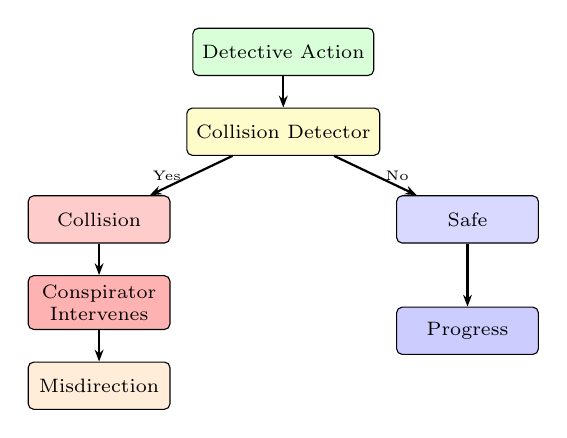
\begin{tikzpicture}[
    node distance=0.35cm,
    box/.style={rectangle, draw, rounded corners=2pt, minimum width=1.8cm, minimum height=0.6cm, align=center, font=\scriptsize},
    arrow/.style={-{Stealth[length=1.5mm]}, thick},
]

\node[box, fill=green!15] (action) {Detective Action};
\node[box, fill=yellow!20, below=0.4cm of action] (check) {Collision Detector};
\node[box, fill=red!20, below left=0.5cm and 0.2cm of check] (collision) {Collision};
\node[box, fill=blue!15, below right=0.5cm and 0.2cm of check] (safe) {Safe};
\node[box, fill=red!30, below=0.4cm of collision] (intervene) {Conspirator\\Intervenes};
\node[box, fill=orange!15, below=0.4cm of intervene] (misdirect) {Misdirection};
\node[box, fill=blue!20, below=0.8cm of safe] (progress) {Progress};

\draw[arrow] (action) -- (check);
\draw[arrow] (check) -- node[left, font=\tiny] {Yes} (collision);
\draw[arrow] (check) -- node[right, font=\tiny] {No} (safe);
\draw[arrow] (collision) -- (intervene);
\draw[arrow] (intervene) -- (misdirect);
\draw[arrow] (safe) -- (progress);

\end{tikzpicture}
\caption{Collision detection: when the detective approaches truth, conspirators intervene to maintain the cover-up.}
\label{fig:collision}
\end{figure}


% ============================================================
% Figure 3: Dual-Layer Narrative (Single Column)
% ============================================================
\begin{figure}[t]
\centering
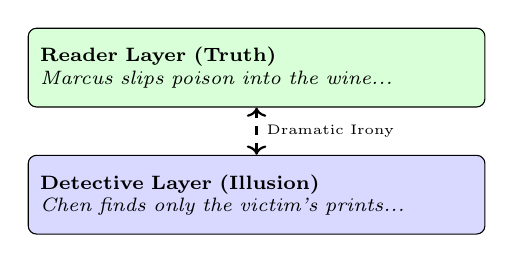
\begin{tikzpicture}[
    node distance=0.3cm,
    layer/.style={rectangle, draw, rounded corners=3pt, minimum width=5.8cm, minimum height=1cm, align=left, font=\scriptsize, text width=5.5cm},
    arrow/.style={-{Stealth[length=1.5mm]}, thick, dashed},
]

\node[layer, fill=green!15] (reader) {
    \textbf{Reader Layer (Truth)}\\
    \textit{Marcus slips poison into the wine...}
};

\node[layer, fill=blue!15, below=0.6cm of reader] (detective) {
    \textbf{Detective Layer (Illusion)}\\
    \textit{Chen finds only the victim's prints...}
};

\draw[arrow, <->] (reader.south) -- node[right, font=\tiny] {Dramatic Irony} (detective.north);

\end{tikzpicture}
\caption{Dual-layer structure creates dramatic irony: readers know the truth while watching the detective be misled.}
\label{fig:dual-layer}
\end{figure}


% ============================================================
% Figure 4: Horizontal Flow (Alternative - Very Compact)
% ============================================================
\begin{figure}[t]
\centering
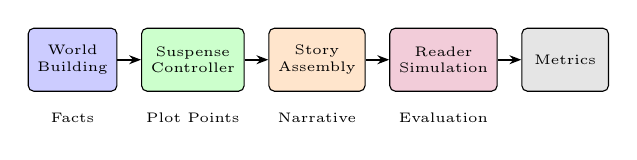
\begin{tikzpicture}[
    node distance=0.15cm,
    box/.style={rectangle, draw, rounded corners=2pt, minimum width=1.1cm, minimum height=0.8cm, align=center, font=\tiny},
    arrow/.style={-{Stealth[length=1.5mm]}, thick},
]

\node[box, fill=blue!20] (p1) {World\\Building};
\node[box, fill=green!20, right=0.3cm of p1] (p2) {Suspense\\Controller};
\node[box, fill=orange!20, right=0.3cm of p2] (p3) {Story\\Assembly};
\node[box, fill=purple!20, right=0.3cm of p3] (p4) {Reader\\Simulation};
\node[box, fill=gray!20, right=0.3cm of p4] (out) {Metrics};

\draw[arrow] (p1) -- (p2);
\draw[arrow] (p2) -- (p3);
\draw[arrow] (p3) -- (p4);
\draw[arrow] (p4) -- (out);

% Labels below
\node[below=0.15cm of p1, font=\tiny, align=center] {Facts};
\node[below=0.15cm of p2, font=\tiny, align=center] {Plot Points};
\node[below=0.15cm of p3, font=\tiny, align=center] {Narrative};
\node[below=0.15cm of p4, font=\tiny, align=center] {Evaluation};

\end{tikzpicture}
\caption{Compact pipeline overview.}
\label{fig:pipeline-compact}
\end{figure}
